\documentclass{beamer}
\usetheme[block=fill]{metropolis}

\usepackage{hyperref}
\usepackage{tikz}

\DeclareMathOperator{\M}{\mathcal M}
\DeclareMathOperator{\N}{\mathcal N}
\DeclareMathOperator{\G}{\mathcal G}

\newcommand{\eq}[1]{\begin{align*} #1 \end{align*}}
\newcommand{\game}[8]{\eq{\begin{array}{ccccccccc} \text{I} & #1 && #3 && #5 && #7\\ \text{II} && #2 && #4 && #6 && #8 \end{array}}}

\title[Virtual Set Theory]{Virtual Set Theory\\ {\small\textsc{PhD Defense}}}
\author[Dan Saattrup Nielsen]{Dan Saattrup Nielsen\\ University of Bristol}
\date{September 1, 2020}

\begin{document}

\begin{frame}
	\titlepage
\end{frame}

\begin{frame}{Before we start}

  Note that I will only include \textit{some} results from my thesis here because of time constraints, and have thus left out entire sections of the thesis.

\end{frame}

%%% WHAT IS A VIRTUAL LARGE CARDINAL? %%%
\begin{frame}{An overview of the talk}
  \begin{itemize}
    \item<alert@2> What is a virtual large cardinal?
    \item How do the virtuals interact with each other?
    \item How indestructible are the virtuals?
    \item How do the virtuals relate to other mathematical objects?
      \begin{itemize}
        \item Infinite games
        \item Ideals
      \end{itemize}
  \end{itemize}
\end{frame}

\begin{frame}{What is a virtual large cardinal?}

  Many large cardinals are defined as the \alert{critical point} of an elementary embedding from the universe $V$ into a transitive $\N$.

  \begin{center}
    \begin{tikzpicture}

      % Models
      \draw (0,0) -- (0,3);
      \draw (4,0) -- (4,3);
      \fill (0,-0.3) node {$V$};
      \fill (4,-0.3) node {$\N$};

      % Embedding 
      \draw[->] (0.4,-0.3) -- (3.6,-0.3);
      \fill (2,-0.1) node {$\pi$};
      \draw[|->] (0.3,1) -- (3.7,2);
      \draw (-0.1,1) -- (0.1,1);
      \draw (3.9,2) -- (4.1,2);
      \fill (-0.3,1) node {$\kappa$};
      \fill (4.6,2) node {$\pi(\kappa)$};
    

    \end{tikzpicture}
  \end{center}

\end{frame}

\begin{frame}{What is a virtual large cardinal?}

  We can weaken this large cardinal definition to merely requiring the elementary embedding and target model to exist in a \alert<1>{generic extension} (of $V$).

  \begin{center}
    \begin{tikzpicture}

      % Models
      \draw (0,0) -- (0,3);
      \draw (4,0) -- (4,3);
      \fill (0,-0.3) node {$V$};
      \fill (4.6,-0.3) node {$\N\in V[g]$};

      % Embedding 
      \draw[->] (0.4,-0.3) -- (3.6,-0.3);
      \fill (2,0) node {$\pi\in V[g]$};
      \draw[|->] (0.3,1) -- (3.7,2);
      \draw (-0.1,1) -- (0.1,1);
      \draw (3.9,2) -- (4.1,2);
      \fill (-0.3,1) node {$\kappa$};
      \fill (4.6,2) node {$\pi(\kappa)$};
    

    \end{tikzpicture}
  \end{center}

  \visible<2>{We have two variants of such cardinals.}

\end{frame}

\begin{frame}{What is a virtual large cardinal?}

  The \alert<1>{faint} large cardinals are the ones where the embedding goes from \alert<1>{$H_\theta^V$}, for some regular uncountable $\theta$.

  \begin{center}
    \begin{tikzpicture}

      % Models
      \draw (0,0) -- (0,3);
      \draw (4,0) -- (4,3);
      \fill (0,-0.3) node {$\alert<1>{H_\theta^V}$};
      \fill (4.6,-0.3) node {$\N\in V[g]$};

      % Embedding 
      \draw[->] (0.4,-0.3) -- (3.6,-0.3);
      \fill (2,0) node {$\pi\in V[g]$};
      \draw[|->] (0.3,1) -- (3.7,2);
      \draw (-0.1,1) -- (0.1,1);
      \draw (3.9,2) -- (4.1,2);
      \fill (-0.3,1) node {$\kappa$};
      \fill (4.6,2) node {$\pi(\kappa)$};
    

    \end{tikzpicture}
  \end{center}

  \visible<2->{\alert<2>{Successor cardinals} can be faint large cardinals.}

  \visible<3>{For instance, $\omega_1$ can carry a precipitous ideal.}

\end{frame}

\begin{frame}{What is a virtual large cardinal?}

  The \alert<1>{virtual} large cardinals are faint large cardinals where the target model is a subset of $V$.

  \begin{center}
    \begin{tikzpicture}

      % Models
      \draw (0,0) -- (0,3);
      \draw (4,0) -- (4,3);
      \fill (0,-0.3) node {$H_\theta^V$};
      \fill (4.6,-0.3) node {$\N \alert<1>{\subseteq V}$};

      % Embedding 
      \draw[->] (0.4,-0.3) -- (3.6,-0.3);
      \fill (2,0) node {$\pi\in V[g]$};
      \draw[|->] (0.3,1) -- (3.7,2);
      \draw (-0.1,1) -- (0.1,1);
      \draw (3.9,2) -- (4.1,2);
      \fill (-0.3,1) node {$\kappa$};
      \fill (4.6,2) node {$\pi(\kappa)$};
    

    \end{tikzpicture}
  \end{center}

  \visible<2->{These cardinals are always \alert<2>{1-iterable}.}

  \visible<3>{In particular, \alert<3>{weakly compact} and \alert<3>{inaccessible}.}

\end{frame}

\begin{frame}{What is a virtual large cardinal?}

  In our definitions of virtually $\theta$-strongs and $\theta$-supercompacts, we require that $\pi(\kappa)>\theta$. 

  \visible<2->{This is automatic for strongs and supercompacts in the ``real world'', but the proof uses the Kunen inconsistency, which is not available in the virtual world.}

  \visible<3->{We attach a \alert<3>{pre-} prefix to our virtual large cardinals when we do not require this property.}
  
  \visible<4->{For instance, $\kappa$ is \alert<4>{virtually $\theta$-prestrong} if it is the critical point of a generic $\pi\colon H_\theta^V\to\N$, where $\N\subseteq V$ and $H_\theta^V\subseteq\N$.}

\end{frame}

\begin{frame}{What is a virtual large cardinal?}

  All the virtuals (and faints) are \alert{weak versions} of their ``real'' counterparts.

  \begin{center}
    \begin{tikzpicture}

      % Main vertical line
      \draw (0,0) -- (0,5);

      % L horisontal line
      \draw[dashed] (-1,1.5) -- (4.5,1.5);
      \fill[anchor=west] (3,1.7) node {\footnotesize V = L};

      % 0=1 horisontal line
      \draw[dashed] (-1,4.3) -- (4.5,4.3);
      \fill[anchor=west] (3,4.5) node {\footnotesize 0 = 1};

      % Inaccessible
      \draw (-0.1,0.1) -- (0.1,0.1);
      \fill[anchor=west] (0.2,0.1) node {\small Inaccessible};

      % Weakly compact
      \draw (-0.1,0.6) -- (0.1,0.6);
      \fill[anchor=west] (0.2,0.6) node {\small Weakly compact};

      % Virtuals
      \draw (-0.1,1.1) -- (0.1,1.1);
      \fill[anchor=west] (0.2,1.1) node {\small \alert<1>{Virtual}};

      % Measurable
      \draw (-0.1,1.9) -- (0.1,1.9);
      \fill[anchor=west] (0.2,1.9) node {\small Measurable};

      % Strong
      \draw (-0.1,2.4) -- (0.1,2.4);
      \fill[anchor=west] (0.2,2.4) node {\small Strong};

      % Woodin
      \draw (-0.1,2.9) -- (0.1,2.9);
      \fill[anchor=west] (0.2,2.9) node {\small Woodin};

      % Supercompact
      \draw (-0.1,3.4) -- (0.1,3.4);
      \fill[anchor=west] (0.2,3.4) node {\small Supercompact};

      % Vopenka
      \draw (-0.1,3.9) -- (0.1,3.9);
      \fill[anchor=west] (0.2,3.9) node {\small Vopenka};

      % Berkeley
      \draw (-0.1,4.7) -- (0.1,4.7);
      \fill[anchor=west] (0.2,4.7) node {\small Berkeley};

    \end{tikzpicture}
  \end{center}

\end{frame}


%%% HOW DO THE VIRTUALS INTERACT WITH EACH OTHER? %%%
\begin{frame}{An overview of the talk}
  \begin{itemize}
    \item What is a virtual large cardinal?
    \item<alert@+> How do the virtuals interact with each other?
    \item How indestructible are the virtuals?
    \item How do the virtuals relate to other mathematical objects?
      \begin{itemize}
        \item Infinite games
        \item Ideals
      \end{itemize}
  \end{itemize}
\end{frame}

\begin{frame}{How do the virtuals interact with each other?}

  Most of the results in this section are comprised in a paper joint with \alert{Dimopoulos} and \alert{Gitman}, and will be submitted within a couple of weeks or so.

\end{frame}

\begin{frame}{How do the virtuals interact with each other? \\
              {\small Strongs and supercompacts}}

  Virtuals behave differently from their real counterparts. The following result from Gitman and Schindler (2018) gave an example of such surprising differences:

  \begin{block}{Theorem (Gitman-Schindler)}
    The following are equivalent for an uncountable cardinal $\kappa$:
    \begin{enumerate}
      \item $\kappa$ is virtually supercompact;
      \item $\kappa$ is virtually strong.
    \end{enumerate}
  \end{block}

\end{frame}

\begin{frame}{How do the virtuals interact with each other? \\
              {\small Strongs and supercompacts}}

  We showed that, in $L$, virtually measurables are either virtually $\omega$-superstrong or virtually strong. This gives the following consistency result:

  \begin{block}{Theorem (N.)}
    The following are equiconsistent for uncountable $\theta$:
    \begin{enumerate}
      \item The existence of a virtually $\theta$-strong cardinal;
      \item The existence of a virtually $\theta$-measurable cardinal.
    \end{enumerate}
  \end{block}

  \only<2>{The reason why we are working in $L$ is that, in $L$, being virtually measurable is equivalent to being virtually prestrong. This can be seen by condensation.}

  \only<3>{Together with the Gitman-Schindler result we thus get that the virtually measurables are equiconsistent with the virtually supercompacts.}

\end{frame}

\begin{frame}{How do the virtuals interact with each other? \\
              {\small Strongs and supercompacts}}

  Our intuition about the prestrongs having to do with the Kunen inconsistency is confirmed by the following result.

  \begin{block}{Theorem (N.)}
    The following are equivalent:
    \begin{enumerate}
      \item There exists an uncountable cardinal $\theta$ and a virtually $\theta$-prestrong cardinal which is not virtually $\theta$-strong;
      \item There exists a \alert<2>{virtually rank-into-rank cardinal}.
    \end{enumerate}
  \end{block}

  \visible<2->{$\kappa$ is \alert<2>{virtually rank-into-rank} if it is the critical point of a generic embedding $\pi\colon H_\theta^V\to H_\theta^V$.}

\end{frame}

\begin{frame}{How do the virtuals interact with each other? \\
              {\small Woodins and Vopenkas}}

  Moving to the Woodins and Vopenkas, these also \textit{almost} form a ``virtual pair'':

  \begin{block}{Theorem (Dimopoulos-Gitman-N.)}
    The following are equivalent for an inaccessible $\kappa$:
    \begin{enumerate}
      \item $\kappa$ is Vopenka;
      \item $\kappa$ is virtually pre-Woodin;
      \item $\kappa$ is faintly pre-Woodin.
    \end{enumerate}
  \end{block}

\end{frame}

\begin{frame}{How do the virtuals interact with each other? \\
              {\small Woodins, Vopenkas and Berkeleys}}

  As for the distinction between the virtually pre-Woodins and virtually Woodins, we begin from another angle. 

  \visible<2->{Letting $\textsf{gVP}$ be the generic analogue of Vopenkas Principle, Gitman and Hamkins (2019) showed the following:

  \begin{block}{Theorem (Gitman-Hamkins)}
    If $0^\sharp$ exists then $\textsf{gVP}$ holds and $\textsf{On}$ is not Mahlo.
  \end{block}}

  \visible<3->{In sharpening the hypothesis, we arrived at the virtual analogue of the \alert<3>{Berkeley cardinals}. 

  \begin{block}{Definition}
    A cardinal $\delta$ is \alert{virtually Berkeley} if to every transitive set $\M$ with $\delta\subseteq\M$, there is a generic elementary $\pi\colon\M\to\M$ with $\text{crit}(\pi)<\delta$, and $\text{crit}(\pi)$ can be chosen arbitrarily large below $\delta$.
  \end{block}}

\end{frame}

\begin{frame}{How do the virtuals interact with each other? \\
              {\small Woodins, Vopenkas and Berkeleys}}

  Gitman and Hamkin's result was then firstly sharpened to these Berkeleys:

  \begin{block}{Theorem (N.)}
    If there exists a virtually Berkeley cardinal then $\textsf{gVP}$ holds and $\textsf{On}$ is not Mahlo.
  \end{block}

  \visible<2->{But in analysing the other direction, an interesting result fell out:

  \begin{block}{Theorem (N.)}
    If there are no virtually Berkeley cardinals then $\textsf{On}$ is virtually pre-Woodin iff $\textsf{On}$ is virtually Woodin.
  \end{block}}

\end{frame}

\begin{frame}{How do the virtuals interact with each other? \\
              {\small Woodins, Vopenkas and Berkeleys}}

  Ultimately this led to the following equivalence, showing Berkeley cardinals to be the optimal hypothesis, as well as showing that the Berkeley cardinals are the \alert<1>{natural analogues} of the virtually rank-into-rank cardinals:

  \begin{block}{Theorem (N.)}
    The following are equivalent: 
    \begin{enumerate}
      \item $\textsf{gVP}$ implies that $\textsf{On}$ is Mahlo;
      \item $\textsf{On}$ is virtually pre-Woodin iff $\textsf{On}$ is virtually Woodin;
      \item There are no virtually Berkeley cardinals.
    \end{enumerate}
  \end{block}

\end{frame}

\begin{frame}{How do the virtuals interact with each other?}
  
  \begin{center}
    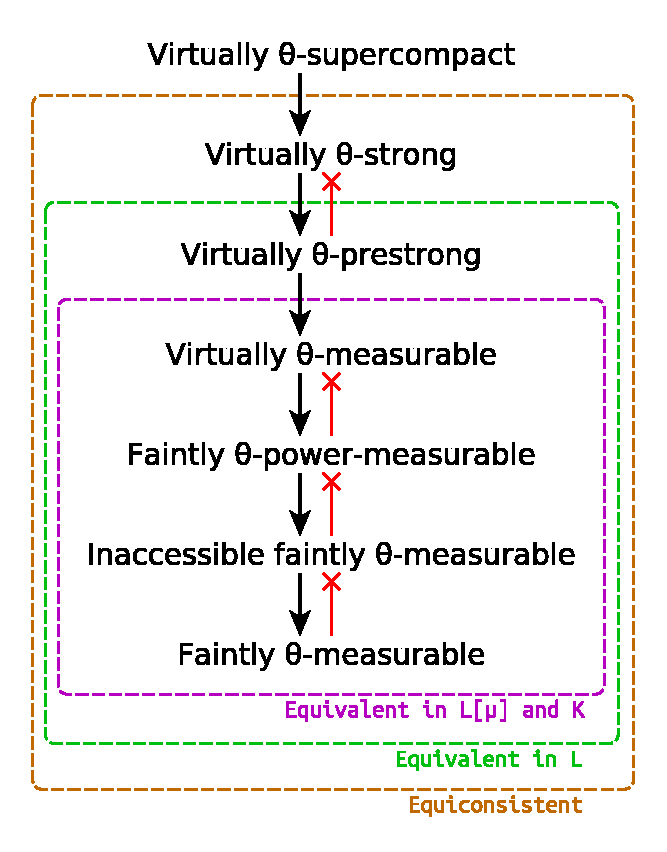
\includegraphics[scale=0.55]{gfx/virtual-separations.pdf}
  \end{center}

\end{frame}


%%% HOW INDESTRUCTIBLE ARE THE VIRTUALS? %%%
\begin{frame}{An overview of the talk}
  \begin{itemize}
    \item What is a virtual large cardinal?
    \item How do the virtuals interact with each other?
    \item<alert@+> How indestructible are the virtuals?
    \item How do the virtuals relate to other mathematical objects?
      \begin{itemize}
        \item Infinite games
        \item Ideals
      \end{itemize}
  \end{itemize}
\end{frame}

\begin{frame}{How indestructible are the virtuals?}

  The results in this section is joint with \alert{Schlicht} and will most likely appear in a joint paper of ours.

\end{frame}

\begin{frame}{How indestructible are the virtuals?}

  We have seen that the virtuals behave differently from their real counterparts, so we can start asking \textit{how} different. 

  \visible<2->{Indestructibility properties of small large cardinals have been widely studied\footnote<2->{\scriptsize Authors include Apter, Cheng, Cody, Cox, Fuchs, Gitman, Hamkins and Johnstone.}, so it would be interesting if we could find a virtual analogue of Laver indestructibility.}

  \visible<3->{After many failed attempts, we strengthened our assumption.

  \begin{block}{Definition (N.-Schlicht)}
    $\kappa$ is \alert<3>{generically setwise $\theta$-supercompact} if it is faintly $\theta$-supercompact, but where the target model is closed under ${<}\theta$-sequences \textit{in the generic extension}.
  \end{block}}

\end{frame}

\begin{frame}{How indestructible are the virtuals?}

  We showed that these exhibit many indestructibility properties:

  \begin{block}{Theorem (N.-Schlicht)}
    Generically setwise supercompact cardinals $\kappa$ are indestructible by:
    \begin{enumerate}
      \item Small forcings;
      \item Adding $\kappa$ many Cohen reals;
      \item ${<}\kappa$-directed closed forcings.
    \end{enumerate}
  \end{block}

  Note that we do \alert{not} require any preparatory forcing.

\end{frame}

\begin{frame}{How indestructible are the virtuals?}

  This is all great, but we feared that the strengthened concept was \textit{too} strong. 

  \visible<2->{We noted firstly that Woodin's countable stationary tower forcing provides an upper consistency bound at a proper class of Woodins, so we at least do not reach the supercompacts.} 

  \visible<3->{Usuba then showed the incredibly surprising result that we are in fact still in the consistency realm among the virtuals:

  \begin{block}{Theorem (Usuba)}
    If $\kappa$ is virtually extendible then $\text{Col}(\omega,{<}\kappa)$ forces that $\omega_1$ is generically setwise supercompact.
  \end{block}}

\end{frame}

\begin{frame}{How indestructible are the virtuals?}

  Despite their weak consistency strength, these cardinals seem to be quite unnatural:

  \begin{block}{Theorem (N.-Schlicht)}
    No cardinal is generically setwise supercompact in either $L$, $K$ below a measurable, or $L[\mu]$ with $\mu$ being a normal ultrafilter.
  \end{block}

\end{frame}


%%% GAMES %%%
\begin{frame}{An overview of the talk}
  \begin{itemize}
    \item What is a virtual large cardinal?
    \item How do the virtuals interact with each other?
    \item How indestructible are the virtuals?
    \item<alert@+> How do the virtuals relate to other mathematical objects?
      \begin{itemize}
        \item<alert@+> Infinite games
        \item Ideals
      \end{itemize}
  \end{itemize}
\end{frame}

\begin{frame}{Infinite games}

  The results in this section are included in a joint paper with \alert{Welch} and is published in the Journal of Symbolic Logic.

\end{frame}

\begin{frame}{Infinite games}

  We now move to set-theoretic \alert<1>{games}.

  \visible<2->{We will be dealing with \alert<2>{weak $\kappa$-models}, being $\kappa$-sized models $\M$ of $\textsf{ZFC}^-$ containing all $\alpha\leq\kappa$.}

  \visible<3->{
    \begin{block}{Definition} 
      We say that an $\M$-measure $\mu$ on $\kappa$ is...
      \begin{itemize}
        \item \alert<3>{$\M$-normal} if $(\M,\in,\mu)\models\forall\vec X\in {^\kappa\mu}\colon\triangle\vec X\in\mu$;
        \item \alert<3>{genuine} if $|\triangle\vec X|=\kappa$ for every $\vec X\in {^\kappa\mu}$;
        \item \alert<3>{normal} if $\triangle\vec X$ is stationary in $\kappa$ for every $\vec X\in {^\kappa\mu}$.
      \end{itemize}
    \end{block}
  }

\end{frame}

\begin{frame}{Infinite games}

  Define the following game \alert<1>{$\G_\gamma^\theta(\kappa)$}:

  \game{\alert<2>{\M_0}}{\alert<3,5>{\mu_0}}{\alert<2>{\M_1}}{\alert<3,5>{\mu_1}}{\dots}{\dots}{\alert<2>{\M_\gamma}}{\alert<3,6>{\mu_\gamma}}

  \visible<2->{The \alert<2>{$\M_\alpha$}'s are \alert<2>{weak $\kappa$-models}}
  \visible<3->{, the \alert<3>{$\mu_\alpha$}'s are \alert<3>{$\M_\alpha$-measures on $\kappa$ with a wellfounded ultrapower}.}

  \visible<4->{All the models and measures are \alert<4>{$\subseteq$-increasing} and we take \alert<4>{unions at limit rounds}.}

  \visible<5->{These measures are \alert<5>{normal} when \alert<5>{$\alpha<\gamma$}}
  \visible<6->{, and \alert<6>{$\mu_\gamma$} is \alert<6>{$\M_\gamma$-normal}.}

  \visible<7->{\alert<7>{Player II wins} iff they can continue playing through all the rounds.}

\end{frame}

\begin{frame}{Infinite games}

  These games lead to the following large cardinals:

  \begin{block}{Definition}
    A cardinal $\kappa$ is \alert<1>{$\gamma$-Ramsey} for $\gamma\leq\kappa$ if player I does not have a winning strategy in $\G_\gamma^\theta(\kappa)$ for all regular $\theta>\kappa$. 

    \visible<2->{Further, $\kappa$ is \alert<2>{strategic $\gamma$-Ramsey} if player II \textit{does} have a winning strategy in the game.}
  \end{block}
  
\end{frame}

\begin{frame}{Infinite games \\ {\small The finite case}}

  We can translate results from Abramson et al (1977) to games and ultrafilters, yielding the following equivalences.

  \begin{block}{Theorem (Abramson et al.)}
    For a cardinal $\kappa=\kappa^{<\kappa}$,
    \begin{itemize}
      \item $\kappa$ is \alert<1>{weakly compact} iff it is \alert<1>{$0$-Ramsey};
      \item $\kappa$ is \alert<1>{weakly ineffable} iff it is \alert<1>{genuine $0$-Ramsey};
      \item $\kappa$ is \alert<1>{ineffable} iff it is \alert<1>{normal $0$-Ramsey};
    \end{itemize}
  \end{block}

  \visible<2->{
  \begin{block}{Theorem (N.)}
    A cardinal $\kappa$ is \alert<2>{completely ineffable} iff it is \alert<2>{coherently ${<}\omega$-Ramsey}, meaning that it is strategic $n$-Ramsey for all $n<\omega$, and the strategies agree with each other.
  \end{block}
  }

\end{frame}

\begin{frame}{Infinite games \\ {\small The countable case}}

  The countable case is when we start making connections back to the virtual large cardinals:

  \begin{block}{Theorem (N.-Schindler)}
    In $L$, the following are equivalent for a cardinal $\kappa$:
    \begin{itemize}
      \item $\kappa$ is strategic $\omega$-Ramsey;
      \item $\kappa$ is virtually measurable.
    \end{itemize}
  \end{block}

\end{frame}


\begin{frame}{Infinite games \\ {\small The countable case}}

  Together with our previous consistency results, we also get the following:

  \begin{block}{Corollary (N.-Schindler)}
    The following are equiconsistent:
    \begin{itemize}
      \item The existence of a strategic $\omega$-Ramsey cardinal;
      \item The existence of a virtually strong cardinal.
    \end{itemize}
  \end{block}

\end{frame}

\begin{frame}{Infinite games \\ {\small The countable case}}

  As we exceed $\omega$, we make a large jump in consistency strength:

  \begin{block}{Theorem (N.)}
    The following are equiconsistent:
    \begin{itemize}
      \item The existence of a strategic $(\omega+1)$-Ramsey cardinal;
      \item The existence of a measurable cardinal.
    \end{itemize}
  \end{block}

  \visible<2->{The proof shows that there is an embedding $\pi\colon V\to\N$ in a $\text{Col}(\omega,2^\kappa)$-extension of $V$, from which there is a measurable cardinal in an inner model of that extension.}

\end{frame}

\begin{frame}{Infinite games \\ {\small The uncountable case}}

  Welch and Schindler also showed that at the uncountable stage, the strategic Ramseys become measurable in $K$:

  \begin{block}{Theorem (Welch)}
    If $0^\P$ does not exist then every strategic $\omega_1$-Ramsey cardinal is measurable in $K$.
  \end{block}

  \begin{block}{Theorem (Schindler)}
    If there is no inner model with a Woodin cardinal then every strategic $\omega_1$-Ramsey cardinal is measurable in $K$.
  \end{block}

\end{frame}


%%% IDEALS %%%
\begin{frame}{An overview of the talk}
  \begin{itemize}
    \item What is a virtual large cardinal?
    \item How do the virtuals interact with each other?
    \item How indestructible are the virtuals?
    \item How do the virtuals relate to other mathematical objects?
      \begin{itemize}
        \item Infinite games
        \item<alert@+> Ideals
      \end{itemize}
  \end{itemize}
\end{frame}

\begin{frame}{Ideals}

  The study of embeddings lying in generic extensions started back in Galvin et al (1978) with the study of \alert<1>{precipitous ideals}.

  Having an ideal at hand gives much more control over the embedding, as we can work more directly with the measures, so it is convenient when we can work with such ideals instead of the generic measures. 

  \visible<2->{This last part of the thesis is an initial analysis of \alert<2>{when} we automatically get such ideals at our disposal.}

  \visible<3->{
  \begin{block}{Definition (N.)} 
    A poset property $\Phi(\kappa)$ is \alert<3>{ideal-absolute} if whenever there is a $\Phi(\kappa)$ forcing extension $V[g]$ containing a generic $V$-measure on $\kappa$, then there is an ideal $I\in V$ on $\kappa$ such that $\mathcal P(\kappa)/I$ is forcing equivalent to a forcing satisfying $\Phi(\kappa)$.
  \end{block}
  }

\end{frame}

\begin{frame}{Ideals}

  We first note that a few standard forcing properties are ideal absolute:

  \begin{block}{Proposition (Folklore)}
    ``$\kappa^+$-chain condition'' is ideal-absolute.
  \end{block}

  \begin{block}{Theorem (N.)}
    ``${<}\lambda$-distributivity'' is ideal-absolute for regular $\lambda\in[\omega,\kappa^+]$.
  \end{block}

\end{frame}

\begin{frame}{Ideals}

  The main result of the section is then the following, which builds upon and improves an unpublished result due to Foreman:

  \begin{block}{Theorem (Foreman-N.)}
    Let $\kappa$ and $\lambda\leq\kappa^+$ be regular cardinals. If player II has a winning strategy in \alert<2>{$\G_\lambda^-(\kappa)$} then $\kappa$ carries a $\kappa$-complete normal ideal $I$ such that $\mathcal P(\kappa)/I$ is $(\kappa,\kappa)$-distributive and has a dense ${<}\lambda$-closed subset.
  \end{block}

  \visible<2->{
  Here \alert<2>{$\G_\lambda^-(\kappa)$} is the same game as $\G_\lambda^\theta(\kappa)$ for any $\theta$, but where we do not require the final measure to have a wellfounded ultrapower.
  }

\end{frame}

\begin{frame}{Ideals}

  Using our previous game-theoretic results, we get the following two corollaries.

  \begin{block}{Corollary (N.)}
    ``$(\kappa,\kappa)$-distributive ${<}\lambda$-closed'' is ideal-absolute for regular $\lambda\in[\omega,\kappa^+]$.
  \end{block}

  \begin{block}{Corollary (N.)}
    ``${<}\lambda$-closed $\lambda$-sized'' is ideal-absolute for regular $\lambda\in[\omega,\kappa]$ such that $2^{<\theta}<\kappa$ for every $\theta<\lambda$.
  \end{block}

\end{frame}


%%% THE END %%%
\begin{frame}{The end}

  \begin{center}
    Thank you for your attention.
  \end{center}

\end{frame}


\end{document}
